% \documentclass{book}

\documentclass[12pt]{article}
\usepackage[pdfborder={0 0 0.5 [3 2]}]{hyperref}%
\usepackage[left=1in,right=1in,top=1in,bottom=1in]{geometry}%
\usepackage[shortalphabetic]{amsrefs}%
\usepackage{amsmath}
\usepackage{enumerate}
\usepackage{enumitem}
\usepackage{amssymb}                
\usepackage{amsmath}                
\usepackage{amsfonts}
\usepackage{amsthm}
\usepackage{bbm}
\usepackage[table,xcdraw]{xcolor}
\usepackage{tikz}
\usepackage{float}
\usepackage{booktabs}
\usepackage{svg}
\usepackage{mathtools}
\usepackage{cool}
\usepackage{url}
\usepackage{graphicx,epsfig}
\usepackage{makecell}
\usepackage{array}

\def\noi{\noindent}
\def\T{{\mathbb T}}
\def\R{{\mathbb R}}
\def\N{{\mathbb N}}
\def\C{{\mathbb C}}
\def\Z{{\mathbb Z}}
\def\P{{\mathbb P}}
\def\E{{\mathbb E}}
\def\Q{\mathbb{Q}}
\def\ind{{\mathbb I}}

\begin{document}
\subsubsection*{Problem 2}In this problem, we use the Fourier collocation method on the following nonlinear PDE:
\[
u_t + (\cos{x})u_x = 0
\]
The problem is defined on the the interval $[0, 2 \pi]$, and we use periodic boundary conditions. We use the Fourier collocation method on two equivalent versions of the PDE problem:
\begin{enumerate}
	\item PDE version 1: $u_t + (\cos{x})u_x = 0$
	\item PDE version 2: $u_t + \frac{1}{2} (\cos{x}) u_x + \frac{1}{2} [( \cos{x}) u]_x - \frac{1}{2} (\cos{x})' u = 0$
\end{enumerate}
We will use each version on two different initial conditions:
\begin{enumerate}
	\item $u(x, 0) = \sin{x}$. Smooth initial condition
	\item $u(x, 0) = x = \pi$. Sawtooth wave (extended periodically)
\end{enumerate}
Time-stepping is done with a fourth-order Runge-Kutta scheme. For error analysis, we look at the L2 error for both versions using different grid sizes. L2 error is computed using Gaussian quadrature for numerical integration. Since we only have the approximate solution at the grid points, we interpolate it using the trigonometric Lagrange polynomials before integration. The exact solution was found using Mathematica's DSolve function and/or the method of characteristics. Unless otherwise specified, the numerical scheme was carried out to a time of $t = \pi/2$, and the error was calcualated at that time. A CFL number of 0.01 was used for the numerical scheme.

\subsection*{Smooth initial condition }
Here we use the smooth initial condition $u(x, 0) = \sin{x}$. First, we show plots of the two versions for times $t = 1.0, 2.0, 3.0, 4.0$. 64 grid points are used for these plots.
\begin{figure}[H]
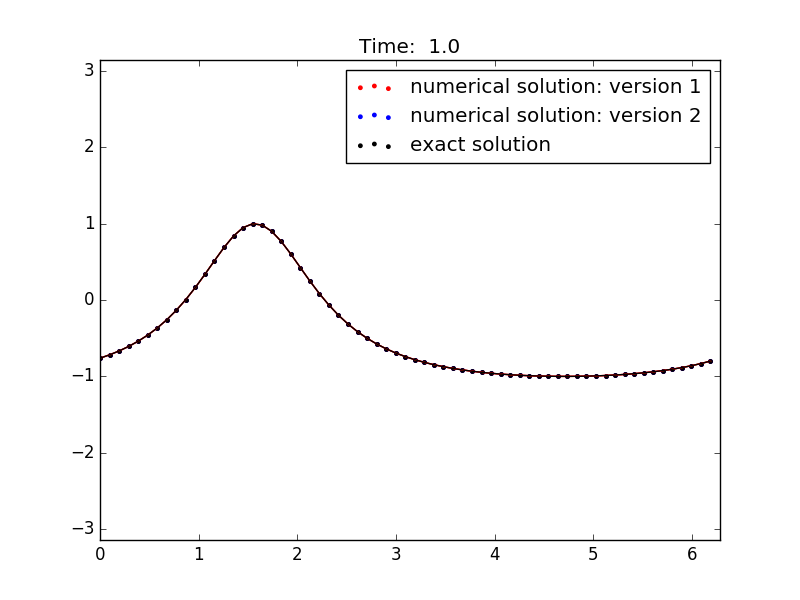
\includegraphics[width=8cm]{images/1frame20.png}
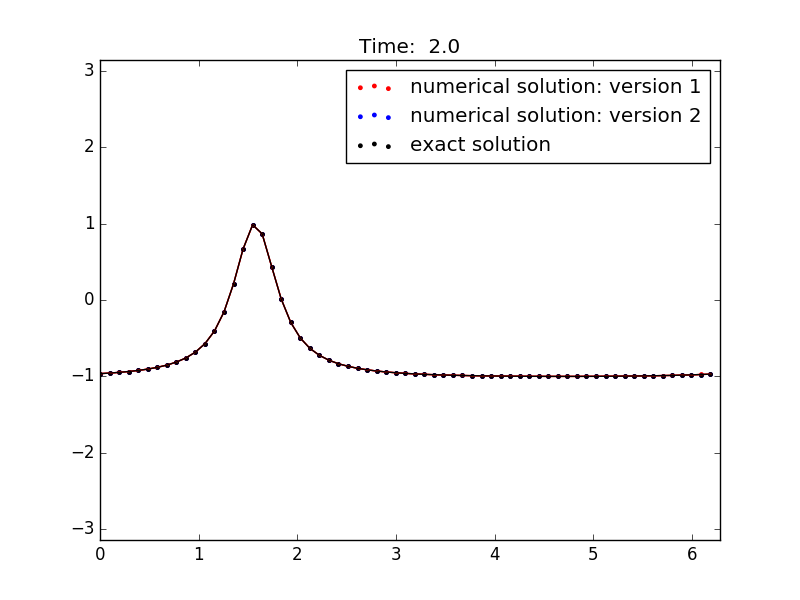
\includegraphics[width=8cm]{images/1frame40.png}
\end{figure}
\begin{figure}[H]
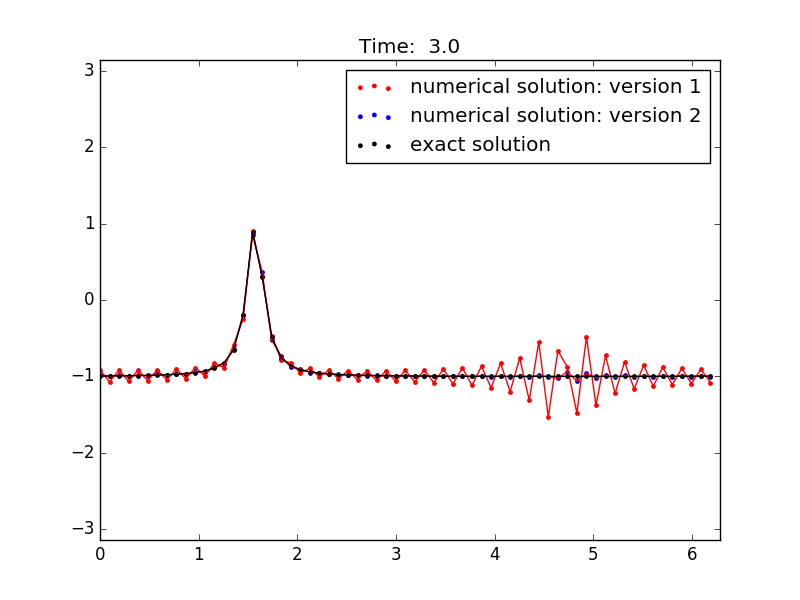
\includegraphics[width=8cm]{images/1frame60.png}
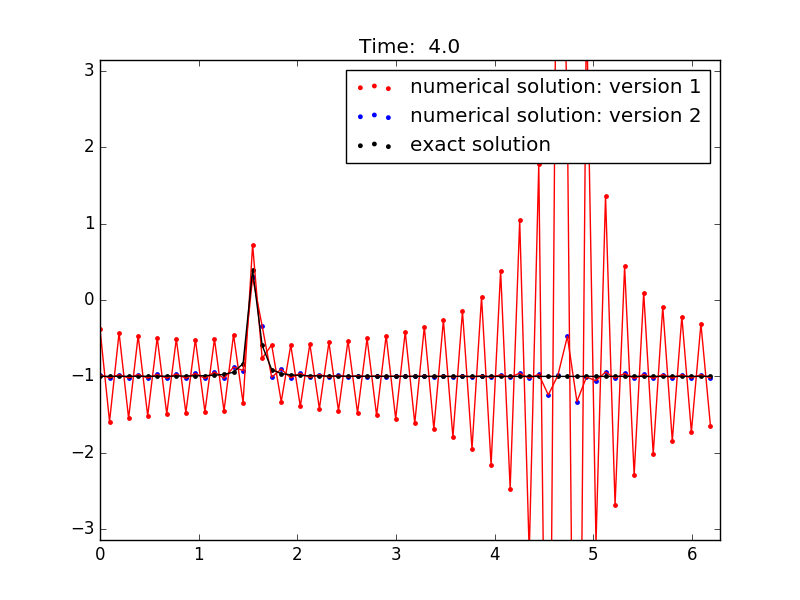
\includegraphics[width=8cm]{images/1frame80.png}
\end{figure}
From visual inspection, both numerical solutions match the exact solution well up to time $t = 2.0$. At $t = 3.0$, we can see that unstable oscillations develop in the numerical solution for version 1. By $t = 4.0$, the unstable oscillations in the numerical solution for version 1 have grown large, and we can start to see unstable oscillations develop in the numerical solution for version 2. We expect version 2 to be more stable given what we proved in class.\\

For the error, we run the numerical method until time $t = \pi/2$ for grid sizes of 4, 8, 16, 32, 64, and 128. Output from the program is given below.
\begin{figure}[H]
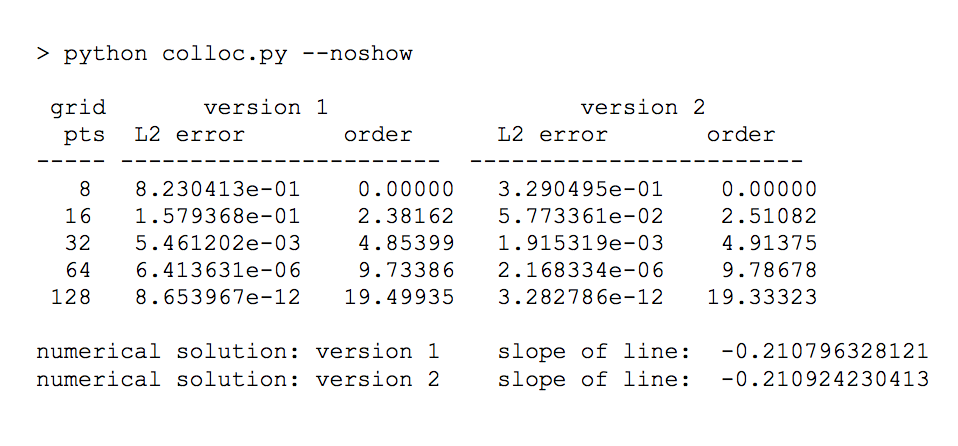
\includegraphics[width=15cm]{images/colloc-output.png}
\end{figure}

Since the orders increase in both cases, we suspect that the L2 error decays exponentially as a function of grid size. We confirm this by plotting L2 error vs. the log of the grid size; the points lie approximately on a straight line in this plot, which is shown below. The exponential decay constant in both cases is approximately 0.21, which is the slope of the best-fit straight line for these plots.
\begin{figure}[H]
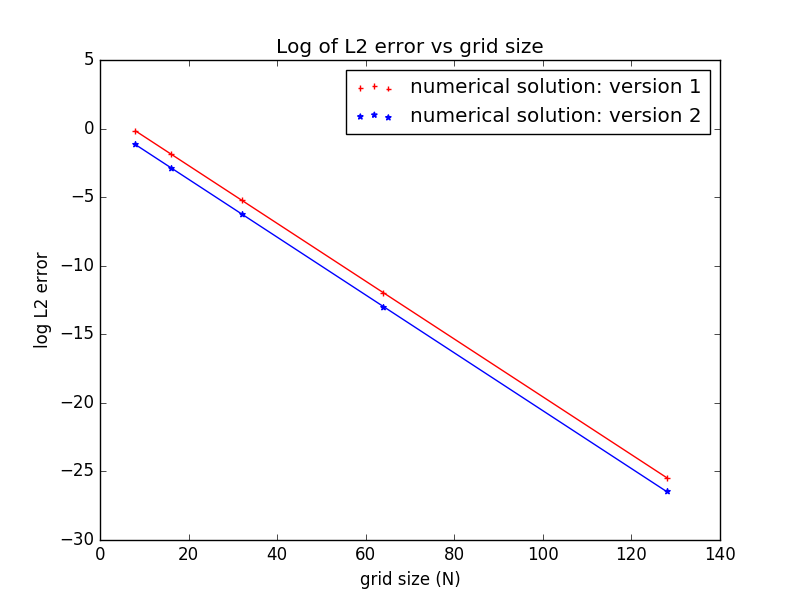
\includegraphics[width=10cm]{images/1error.png}
\end{figure}

\subsection*{Sawtooth wave}
Here we use the sawtooth wave $u(x, 0) = x = \pi$, which is extended periodically. First, we show plots of the two versions for times $t = 0.25, 0.5, 0.75, 1.0$. 128 grid points are used for these plots.
\begin{figure}[H]
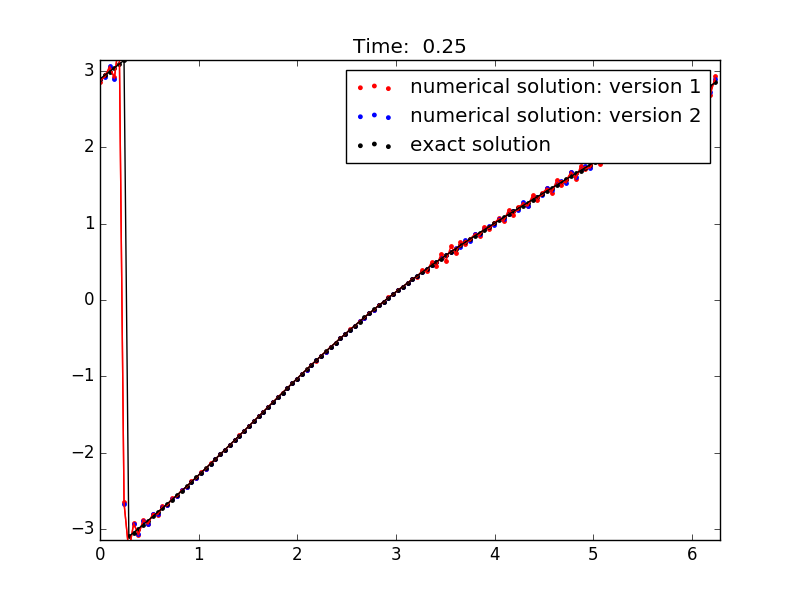
\includegraphics[width=8cm]{images/2frame1.png}
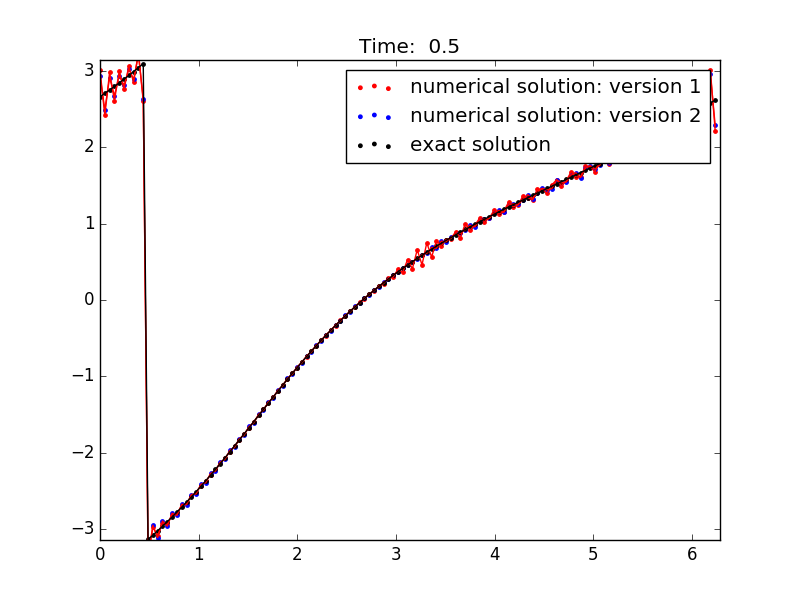
\includegraphics[width=8cm]{images/2frame2.png}
\end{figure}
\begin{figure}[H]
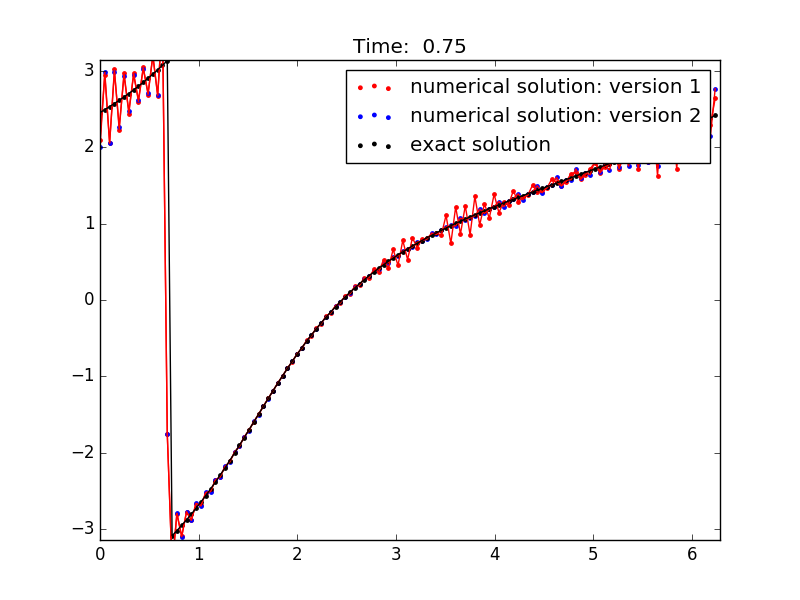
\includegraphics[width=8cm]{images/2frame3.png}
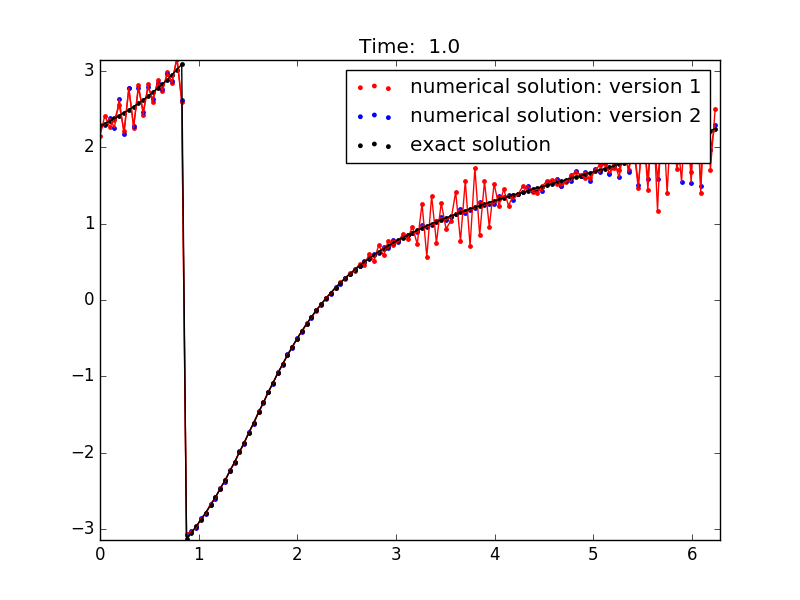
\includegraphics[width=8cm]{images/2frame4.png}
\end{figure}
From this we can see that unstable oscillations develop quickly near the discontinuity in the initial condition. These unstable oscillations develop sooner in version 1 than version 2, although they rapidly take over in both cases. The error in this case is large enough that it we do not have nice relationship between grid size and L2 error, even for small numbers of time steps. In fact, computing the L2 error is difficult in this case, since Gaussian quadrature methods do not perform as well on rapidly oscillating functions. For completeness, the error table for an end time of $t = 0.1$ is given below.

\begin{figure}[H]
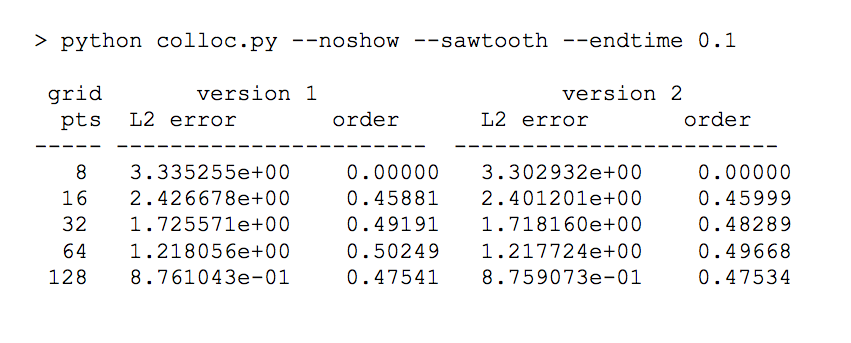
\includegraphics[width=15cm]{images/colloc-output2.png}
\end{figure}

\end{document}

